
\subsection{Maximizing Correlation Using Wall Friction}\label{subsec:ClosedLoopCovarianceControl}
Using the environment to individually move $n$ particles to goal positions in Alg. \ref{alg:PosControlNRobots} requires $O(n^2)$ time, while  Alg. \ref{alg:PosControl2Robots} can only control two particles. The controllers in Section \ref{sec:theory} are efficient because they require only a single move but the range of possible configurations are limited. This section presents an efficient technique to generate desired correlations.

Assume an obstacle-free, bounded, unit-size square workspace. 
 As shown in Fig.~\ref{fig:SquareFill}, the maximum correlation occurs when the swarm is pushed in the direction $\beta = 3\pi/4$. 
 This correlation as a function of swarm area $A$ is never larger than 1/2, and the maximum correlation decays to 0 as $A$ grows to 1. By  \eqref{eq:covAndcorrInSquareWorkspace}, this maximum correlation is:
\begin{align} \label{eq:GravityCorrelation}
\rho_{xy} =  \begin{cases}  \frac{1}{2}  , &  0\le A\le \frac{1}{2}  \\
% \frac{3 A (2 (A-2) A+1)}{4 A \left(A^2+3 \sqrt{2-2 A}-6\right)-12 \sqrt{2-2 A}+17}-1
 \frac{3 A (2 (A-2) A+1)}{4 A^3-24 A+\sqrt{2} (12 A-12) \sqrt{1-A}+17}-1
 , & \frac{1}{2} \le A\le 1
\end{cases}
\end{align}
 If friction obeys the linear boundary layer model of \eqref{eq:boundarylayerflow} with boundary layer thickness $h$ and maximum friction $F_f$ equal to the maximum applied force $F$, we can generate much larger correlations.
Specifically, we can generate correlations larger than 1/2 by using boundary friction if the swarm size is smaller than $\approx 0.43$ and the boundary layer is sufficiently thick. 

 Assume that the swarm is initialized in the lower-left corner, in a rectangle of width $w$ and height $A/w$. 
 Such a rectangular configuration can be accomplished using the variance controllers from \citep{ShahrokhiIROS2015}. 
  If the swarm is then commanded to move a distance $L$ to the right, components of the swarm outside the boundary friction layer of height $h$ move further than components near the boundary. 
   The swarm is contained in a region $R$ composed of no more than three stacked components: at bottom a parallelogram inclined to the right top, at middle a rectangle, and at top a parallelogram inclined to the left top. These regions can be defined by the rectangle's left side, bottom, and top:
\begin{align}
r_{\text{left}} &= \min (L,1-w)\nonumber \\
r_{\text{bottom}} &=\min \left(\frac{A}{w}, h\frac{r_{left}}{L}  \right)\nonumber \\
r_{\text{top}}  &= \min \left(\frac{A}{w}, 1-h\frac{r_{left}}{L}  \right)
\end{align}
If $\frac{A}{w} \le r_{\text{top}}$ the top parallelogram has no area. 
 Similarly, if $r_{\text{top}} \le r_{\text{bottom}}$ the rectangle has no area. 
The mean, variance, and correlation are calculated  using \eqref{eq:meanInSquareWorkspace}, \eqref{eq:varInSquareWorkspace}, and \eqref{eq:covAndcorrInSquareWorkspace} over the region $R$:
\begin{align} \iint_R f(x,y) \, dx \,dy &=  \int_0^{r_{\text{bottom}}}  \int_{\frac{L}{h}y}^{\frac{L}{h}y+w}  f(x,y)  dx \, dy \label{eq:correlationFriction} \\
&+\int_{r_{\text{bottom}}}^{r_{\text{top}}} \int_{r_{\text{left}}}^{r_{\text{left}} +w} f(x,y)    dx \, dy \nonumber\\
&+\int_{r_{\text{top}}}^{\frac{A}{w}} \int_{-\frac{L (y-r_{\text{top}})}{h}+r_{\text{left}}}^{r_{\text{left}}+w-\frac{L (y-r_{\text{top}})}{h}} f(x,y)   dx \, dy \nonumber
\end{align}
 
 Given an environment parameterized by $A$ and $h$, efficient correlation control consists of choosing the $w,L$ pair  that generates the desired positive correlation.
  Negative correlations can be generated by initializing the swarm in the upper left, or lower right.

%freedom is not the freedom to do what we want, but freedom to do what we ought.

% PLACE IN SIMULATION

\subsection{Efficient Control of Correlation}
%A set of simulations were conducted to demonstrate the importance of boundary friction.  
This section examines maximum correlation values as a function of  $w,L$ using \eqref{eq:correlationFriction}
from Section  \ref{subsec:ClosedLoopCovarianceControl}. 
The maximum correlation using boundary layer friction $\displaystyle  \max_{w,L} \left( \rho(A,h,w,L) \right)$ can be found by gradient descent, as shown in Fig.~\ref{fig:ControlledCorrelation}. 
For swarms with small area, this method enables generating the full range of correlations $\pm 1$, while the stable configuration method from Section \ref{sec:theory} could only generate correlations $\pm 1/2$.  As  the swarm area $A$ increases above $\approx 0.43$, the stable configuration method is more effective.
Larger boundary layers $h$ enable more control of correlation.



\begin{figure}
\begin{center}
	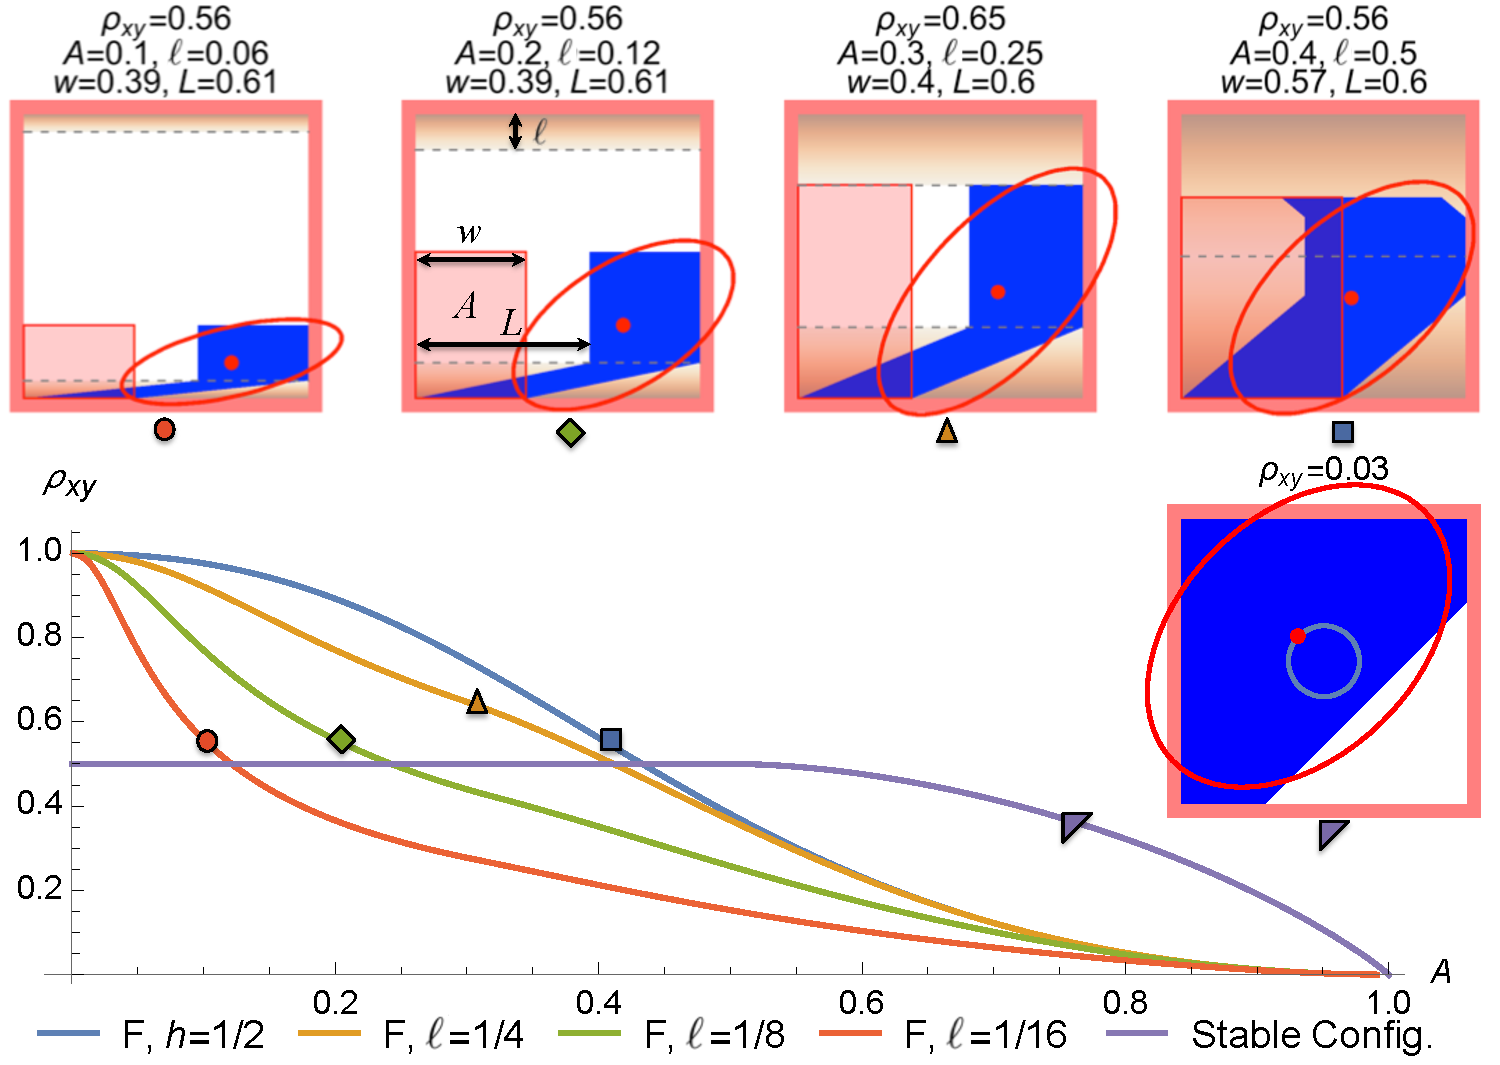
\includegraphics[width=\columnwidth]{ControlledCorrelation.pdf}
\end{center}
\vspace{-1em}
\caption{\label{fig:ControlledCorrelation}
Analytical results comparing maximum correlation under the boundary layer friction model of \eqref{eq:correlationFriction} with four boundary layer thicknesses $h$ and the stable triangular configuration \eqref{eq:GravityCorrelation}.
}
\end{figure}
